\begin{table*}[t]\centering\small
\caption{Synthetic two-agent comparison: five-seed mean system time and boundary waiting (vehicle-minutes). Equal-green fixed baseline is not demand-optimized. These are not METR-LA or real-world results.}
\begin{tabular}{lrrrr}\toprule
Scenario & Fixed system & Responsive system & Fixed waiting & Responsive waiting\\\midrule
Balanced & 3263.3 & 2212.8 & 1.9 & 1.9\\
Arterial peak & 10850.7 & 2840.5 & 4126.1 & 4.6\\
Side peak & 6435.1 & 3173.6 & 629.4 & 3.3\\
Downstream limit & 14308.9 & 6003.9 & 5720.4 & 334.8\\
\bottomrule\end{tabular}\end{table*}
\begin{table*}[t]\centering\small
\caption{Synthetic mean exit throughput and end-of-horizon residuals, vehicles. Fractional values reflect continuum CTM occupancy, not counted individual cars.}
\begin{tabular}{lrrrr}\toprule
Scenario & Fixed exit & Adapt. exit & Fixed left & Adapt. left\\\midrule
Balanced & 1199.8 & 1199.8 & 0.000 & 0.000\\
Arterial peak & 1450.6 & 1450.6 & 0.011 & 0.000\\
Side peak & 1511.0 & 1511.0 & 0.000 & 0.000\\
Downstream limit & 1516.1 & 1520.2 & 4.058 & 0.000\\
\bottomrule\end{tabular}\end{table*}
\begin{figure*}[t]\centering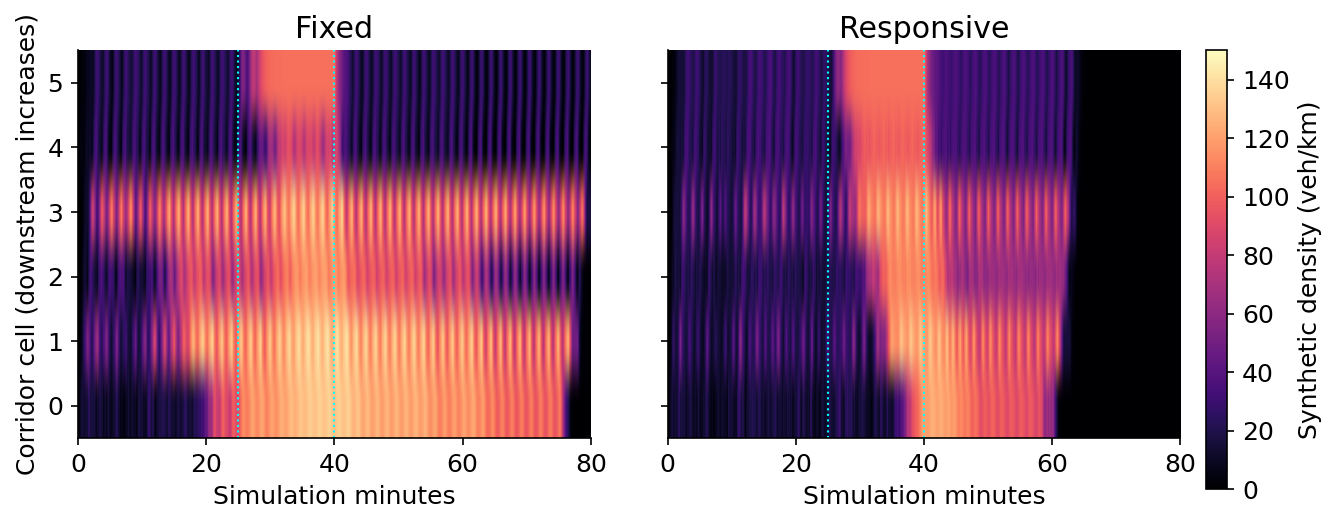
\includegraphics[width=.95\textwidth]{images/control_density.png}
\caption{Synthetic corridor density, downstream-restriction scenario, seed101. Dotted lines bound the reduced exit capacity interval. Density and wave speed are assumed model quantities, not METR-LA measurements.}\end{figure*}
